\documentclass{article}
\usepackage{graphicx}
\usepackage{listings}
\usepackage{ctex}
\usepackage{graphicx}
\usepackage[a4paper, body={18cm,22cm}]{geometry}
\usepackage{amsmath,amssymb,amstext,wasysym,enumerate,graphicx}
\usepackage{float,abstract,booktabs,indentfirst,amsmath}
\usepackage{array}
\usepackage{booktabs} %调整表格线与上下内容的间隔
\usepackage{multirow}
\usepackage{diagbox}
\usepackage{indentfirst}
\usepackage{bm}
\usepackage{fancyhdr}




\pagestyle{fancy}

\lhead{\bfseries \normalsize 学号:1952033\quad 姓名:侯雅玥 \quad 组员:廖宏 \\实验名称:集成运算放大电路的应用\quad 课程名称:电子技术实验\quad 专业:微电子科学与工程 } 
\rhead{}

\begin{document}
	\section{\zihao{4} 实验名称:集成运算放大电路的应用(三)}
    \section{\zihao{4} 实验目的}
    \zihao {5} (1)掌握电压比较器的电路构成及工作原理.\par
               (2)熟悉集成运算放大器的非线性应用,学会比较器的测试方法.
			   \section{\zihao{4} 实验原理}
               电压比较器是集成运放非线性应用电路,它将一个模拟量电压信号和一个参考电压相比较,在两者幅度相等的附近,
               输出电压将产生跃变,相应输出高电平或低电平.比较器可以组成非正弦波形变换电路及应用于模拟与数字信号转换等领域.
               图1所示为一最简单的串联比较型电压比较器$U_R$为参考电压(即比较电压),加在运放的同相输入端,输人电压$U_i$,加在反相输入端.\par
               当$U_i<U_R$时,运放输出高电平,稳压管$D_Z$反向稳压工作,输出端电位被其筘位在稳压管的稳定电压$U_Z$,即$U_o=U_Z$\par 
               当$U_i>U_R$时,运放输出低电平,$D_Z$正向导通,输出电压等于稳压管的正向压降$U_D$,即$U_o=-U_D$\par
               因此,以$U_R$为界,当输入电压Ui变化时,输出端反映出两种状态∶高电位和低电位.表示输出电压与输入电压之间关系的特性曲线,
               称为传输特性.如图2为图1电路的传输特性.\par
               常用的电压比较器有过零比较器、具有滞回特性的比较器、双限比较器(又称窗口比较器)等.\par
               \begin{figure}[h]
                \begin{minipage}[t]{0.5\linewidth} % 如果一行放2个图,用0.5,如果3个图,用0.33  
                  \centering   
                  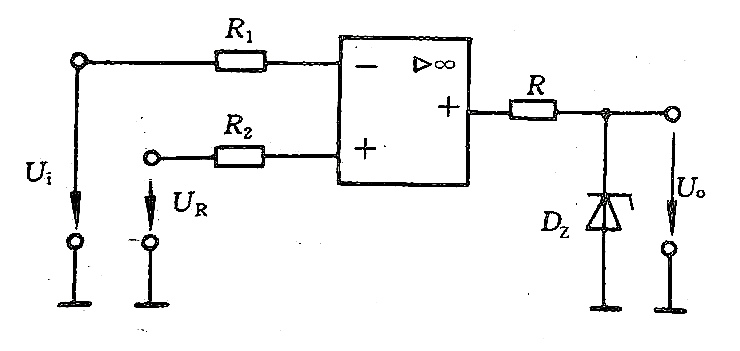
\includegraphics[width=2.5in]{H:/电子技术试验/4-15/4-15-1.jpg}   
                  \caption{电压比较器}   
                  \label{fig:side:a}   
                \end{minipage}%   
                \begin{minipage}[t]{0.5\linewidth}   
                  \centering   
                  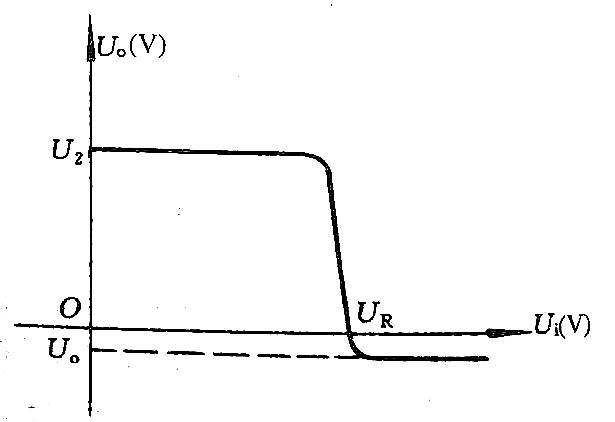
\includegraphics[width=2.5in]{H:/电子技术试验/4-15/4-15-2.jpg}   
                  \caption{传输特性}   
                  \label{fig:side:b}   
                \end{minipage}   
              \end{figure}
              \par
               (1)过零比较器\par
               电路如图3所示为加限幅电路的过零比较器(可用于零电平检测),$D_Z$为限幅稳压管.信号从运放的反相输入端输入;
               比较电压为零(记为$U_C=0V$),从同相端输入。\par
               当$U_i>$0时,输出$U_o=-(U_Z+U_D)$,当$U_i<0$时,$U_o=+(U_Z+U_D)$.其电压传输特性如图4所示.\par
               过零比较器结构简单,灵敏度高,但抗干扰能力差.\par
               \begin{figure}[h]
                \begin{minipage}[t]{0.5\linewidth} % 如果一行放2个图,用0.5,如果3个图,用0.33  
                  \centering   
                  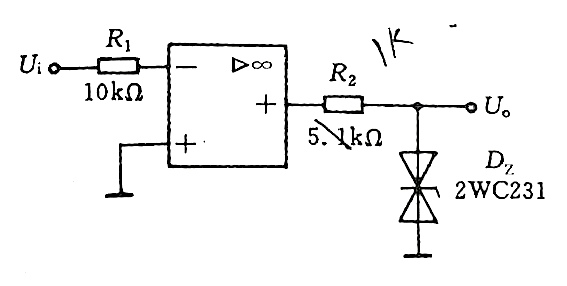
\includegraphics[width=2.5in]{H:/电子技术试验/4-15/4-15-3.jpg}   
                  \caption{过零比较器}   
                  \label{fig:side:a}   
                \end{minipage}%   
                \begin{minipage}[t]{0.5\linewidth}   
                  \centering   
                  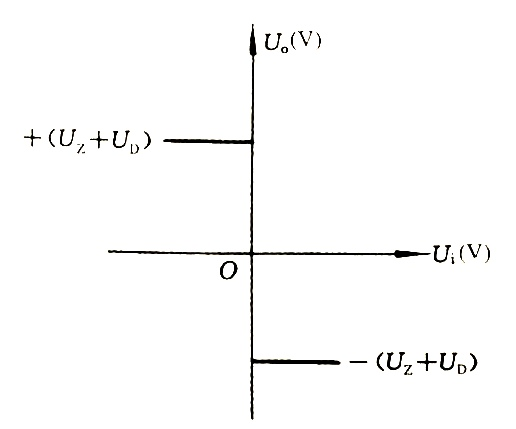
\includegraphics[width=2.5in]{H:/电子技术试验/4-15/4-15-4.jpg}   
                  \caption{传输特性}   
                  \label{fig:side:b}   
                \end{minipage}   
              \end{figure}
              \par
              (2)滞回比较器\par
               图3为滞回比较器.过零比较器在实际工作时,如果$U_i$恰好在过零值附近,则由于零点漂移的存在,$U_o$将不断地由一个极限值
               转换到另一个极限值,这在控制系统中,对执行机构将是很不利的.为此,需要输出特性具有滞回现象,
               如图3所示,从输出端通过一个电阻分压反馈到同相输入端,$\Sigma$ 点电压随$U_o$的大小和极性而改变,使过零点离开原来位置.\par
               $\Sigma$ 点电压为门限电压,它有两个值分别为上门限电压$U_H$和下门限电压$U_L$,差值称门限宽度或回差,
               即 $\Delta U=U_H-U_L$.当$U_o$为正(记作$+U_{om}$),此时$\Sigma$点电压为\[U_H=\frac{R_2}{R_2+R_f}U_{om}\]  \par
               当$U_i>U_H$后,即$U_o$由正变负(记作$-U_{om}$),此时$\Sigma$电压为\[U_L=-\frac{R_2}{R_2+R_f}U_{om}\]  \par
               \begin{figure}[h]
                \begin{minipage}[t]{0.5\linewidth} % 如果一行放2个图,用0.5,如果3个图,用0.33  
                  \centering   
                  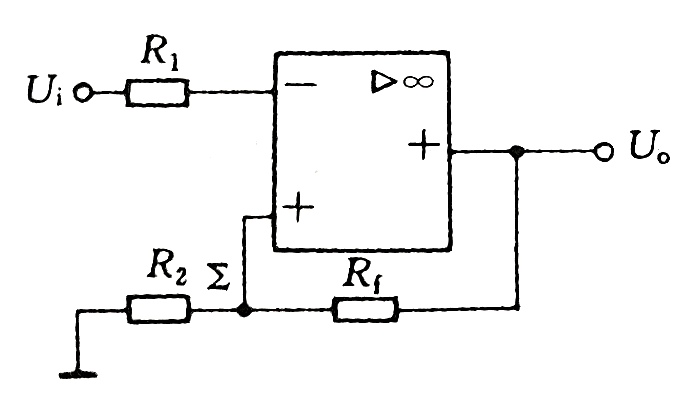
\includegraphics[width=2.5in]{H:/电子技术试验/4-15/4-15-7.jpg}   
                  \caption{滞回比较器}   
                  \label{fig:side:a}   
                \end{minipage}%   
                \begin{minipage}[t]{0.5\linewidth}   
                  \centering   
                  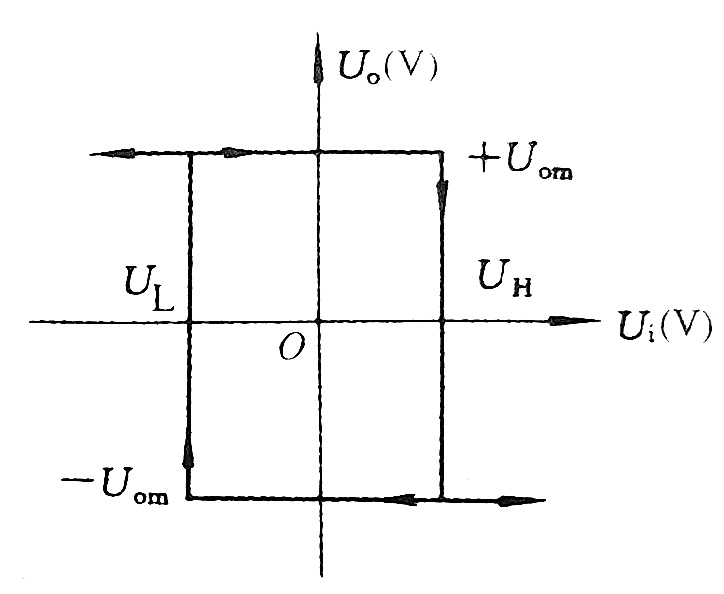
\includegraphics[width=2.5in]{H:/电子技术试验/4-15/4-15-8.jpg}   
                  \caption{传输特性}   
                  \label{fig:side:b}   
                \end{minipage}   
              \end{figure}
              \par
              故只有当$U_i$下降到$U_L$以下,才能使$U_o$再度回升到$+U_{om}$,于是出现图8中所示的滞回特性. 因此,回差为\[\Delta U=\frac{2R_2}{R_2+Rf}U_{om}\]
改变 $R_2$或 $R_f$的数值可以改变回差的大小.\par 
\newpage
\section{\zihao{4} 实验电路}

\begin{figure}[h]
	\begin{minipage}[t]{0.5\linewidth} % 如果一行放2个图,用0.5,如果3个图,用0.33  
	  \centering   
	  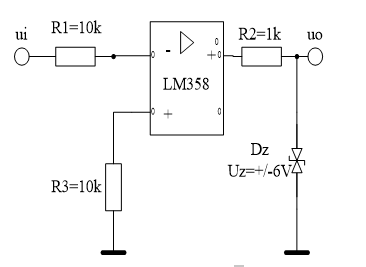
\includegraphics[width=3.2in]{H:/电子技术试验/4-15/4-15-9.png}   
	  \caption{反相过零比较器}   
	  \label{fig:side:a}   
	\end{minipage}%   
	\begin{minipage}[t]{0.5\linewidth}   
	  \centering   
	  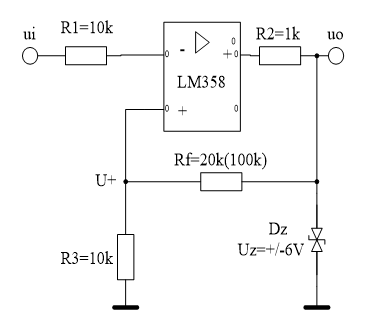
\includegraphics[width=3.2in]{H:/电子技术试验/4-15/4-15-10.png}   
	  \caption{反向滞回比较器}   
	  \label{fig:side:b}   
	\end{minipage}   
  \end{figure}

\begin{figure}[h]
	%\small
	\centering
	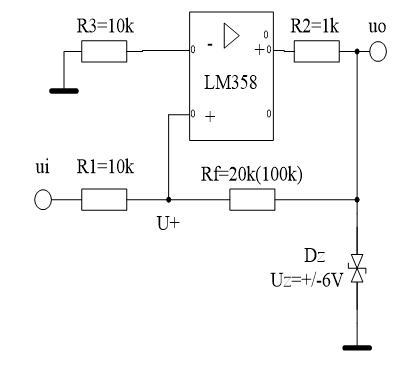
\includegraphics[width=3.2in]{H:/电子技术试验/4-15/4-15-11.png}
	\caption{同相滞回比较器} \label{fig:aa}
\end{figure}
\newpage
\section{\zihao{4} 实验内容及步骤}
(1).按图9接线,输入三角波 f=50Hz Uip-p=12V,用示波器观测并记录Ui、Uo的波形及其电压传输特性曲线。\par
(2).按图10接线,输入三角波 f=50Hz Uip-p=12V,用示波器观测并记录Ui、Uo和U+的波形及其电压传输特性曲线。\par
(3).按图11接线,输入三角波 f=50Hz Uip-p=12V,用示波器观测并记录Ui、Uo和U+的波形及其电压传输特性曲线。\par
	
\section{\zihao{4} 数据处理}
	\subsection {反相过零比较器}
	
	\begin{figure}[h]
		%\small
    \begin{minipage}[t]{0.5\linewidth} % 如果一行放2个图,用0.5,如果3个图,用0.33  

		\centering
		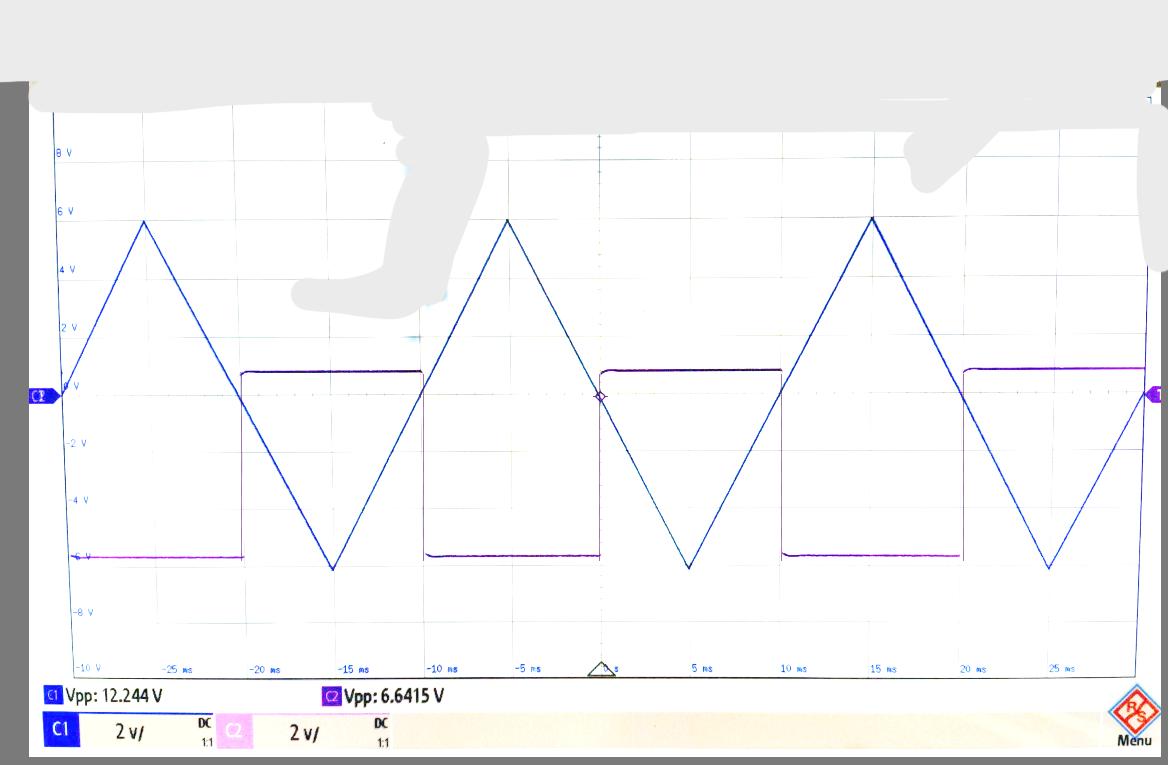
\includegraphics[width=3.5in]{H:/电子技术试验/4-15/4-15-12.png}
		\caption{反相过零比较器Ui和Uo的波形} \label{fig:aa}
  \end{minipage}   
  \begin{minipage}[t]{0.5\linewidth} % 如果一行放2个图,用0.5,如果3个图,用0.33  
		%\small
		\centering
		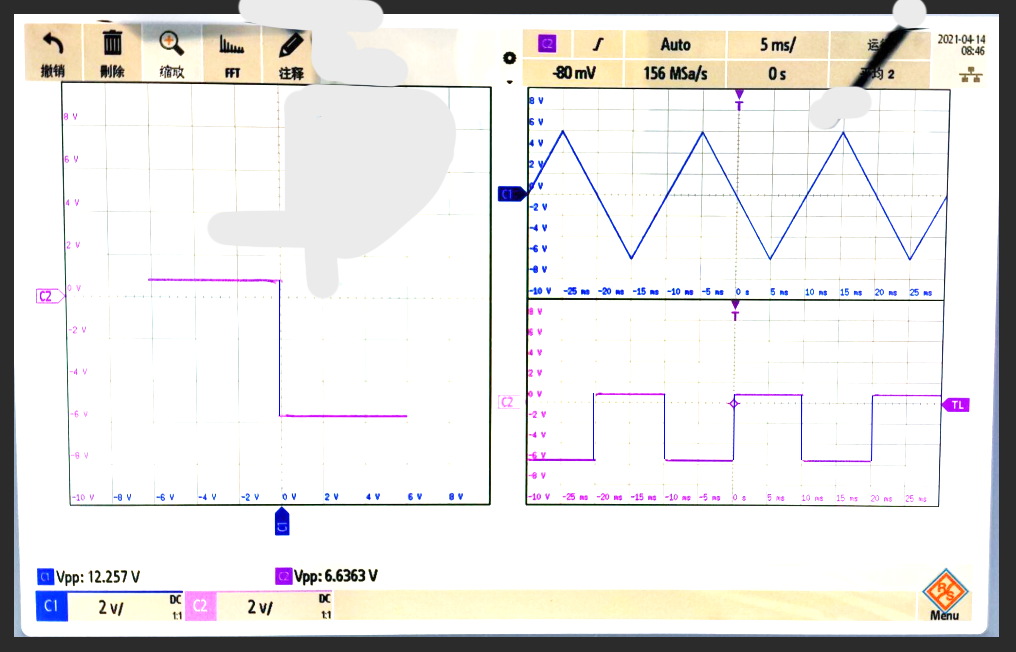
\includegraphics[width=3.5in]{H:/电子技术试验/4-15/4-15-13.png}
		\caption{反相过零比较器的电压传输特性} \label{fig:aa}
  \end{minipage}
  \end{figure}
	\par
\newpage
	\subsection {反相滞回比较器}
    \begin{figure}[h]
      \begin{minipage}[t]{0.5\linewidth} % 如果一行放2个图,用0.5,如果3个图,用0.33  
		\centering
		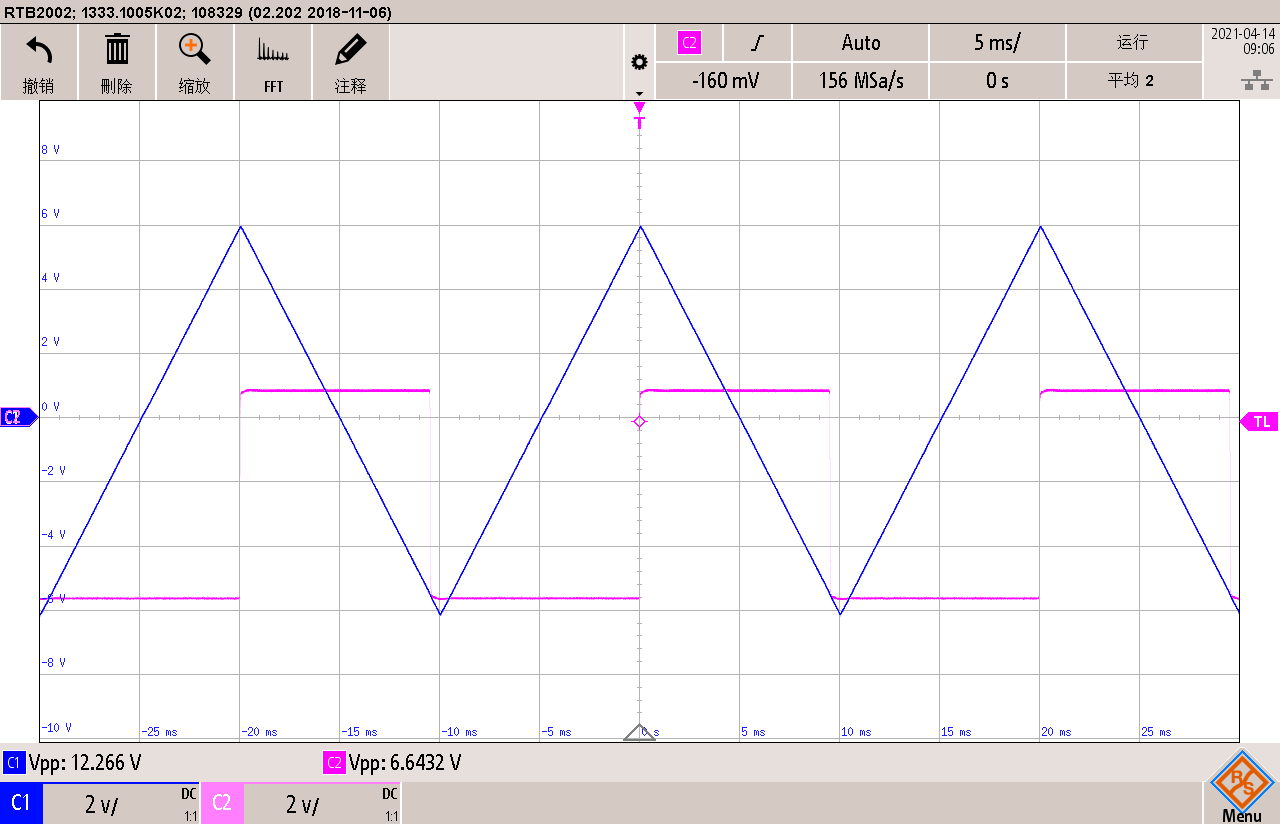
\includegraphics[width=3.5in]{H:/电子技术试验/4-15/4-15-14.png}
		\caption{反相滞回比较器Ui和Uo的波形} \label{fig:aa}
	\end{minipage}
  \begin{minipage}[t]{0.5\linewidth} % 如果一行放2个图,用0.5,如果3个图,用0.33  
		%\small
		\centering
		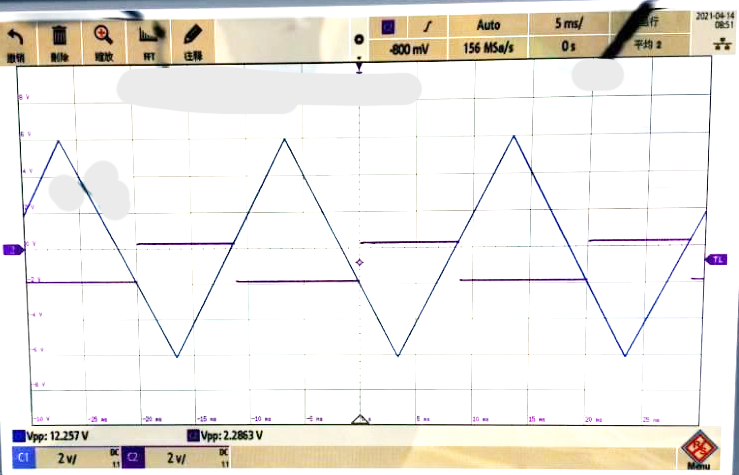
\includegraphics[width=3.5in]{H:/电子技术试验/4-15/4-15-15.png}
		\caption{反相滞回比较器的Ui和U+的波形} \label{fig:aa}
	\end{minipage}
  \end{figure}

    \begin{figure}[h]
		%\small
		\centering
		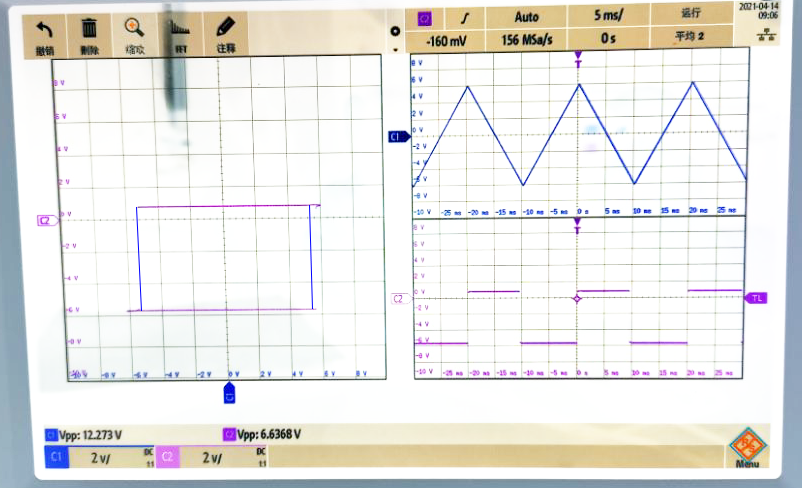
\includegraphics[width=3.5in]{H:/电子技术试验/4-15/4-15-16.png}
		\caption{反相滞回比较器的电压传输特性} \label{fig:aa}
	\end{figure}
	\par
  则反向滞回比较器的门限电压计算:
  \[U_H=\frac{R_3}{R_3+R_f}U_{om}=1.106V\]
  \[U_L=\frac{R_3}{R_3+R_f}U_{om}=-1.106V\]
  回差:
  \[\Delta U=\frac{2R_2}{R_2+R_f}U_{om}=2.212V\]
  \[\delta (\Delta U)=\frac{\Delta U-\Delta U_0}{\Delta U_0}=3.2\%\]
  \newpage
	\subsection {同相比例运算放大器的虚短}
    \begin{figure}[h]
      \begin{minipage}[t]{0.5\linewidth} % 如果一行放2个图,用0.5,如果3个图,用0.33  
		%\small
		\centering
		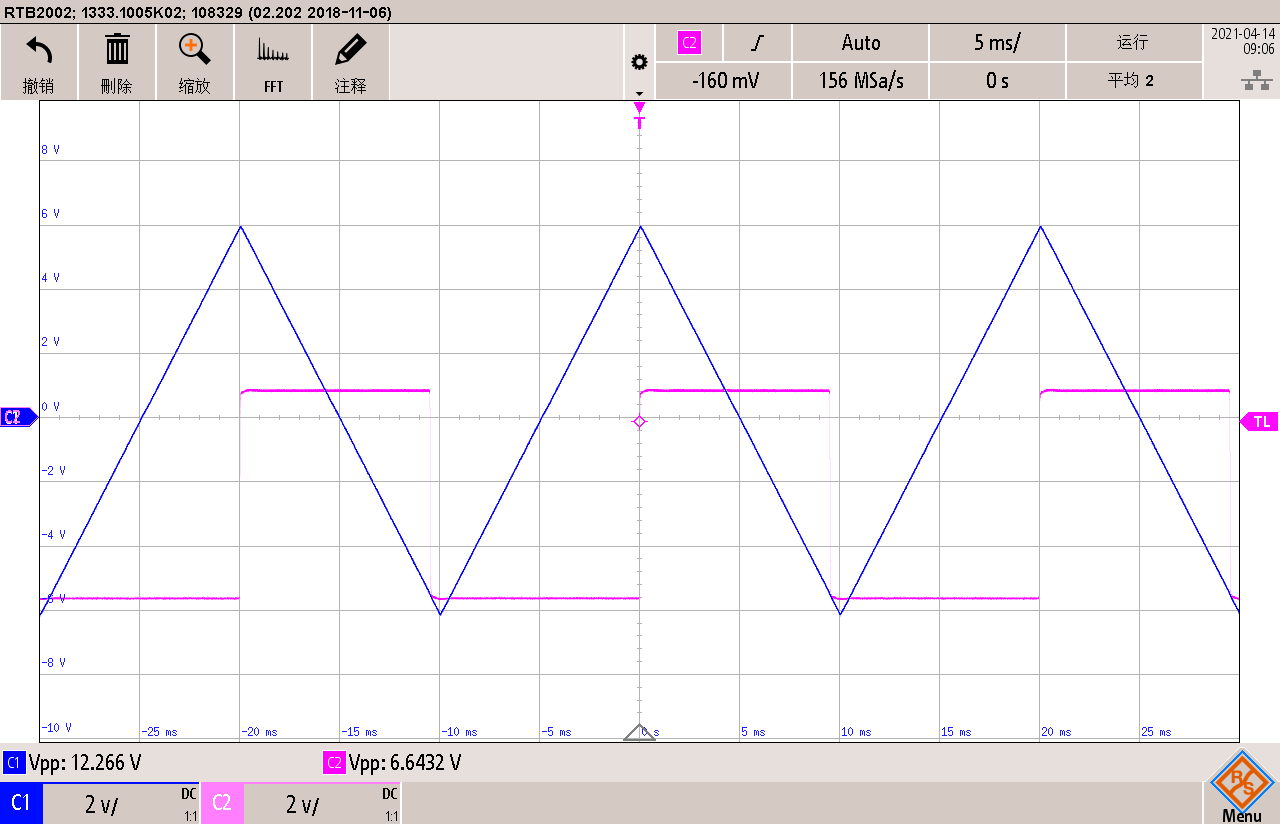
\includegraphics[width=3.5in]{H:/电子技术试验/4-15/4-15-17.png}
		\caption{同相滞回比较器Ui和Uo的波形} \label{fig:aa}
	\end{minipage}
  \begin{minipage}[t]{0.5\linewidth} % 如果一行放2个图,用0.5,如果3个图,用0.33  
		%\small
		\centering
		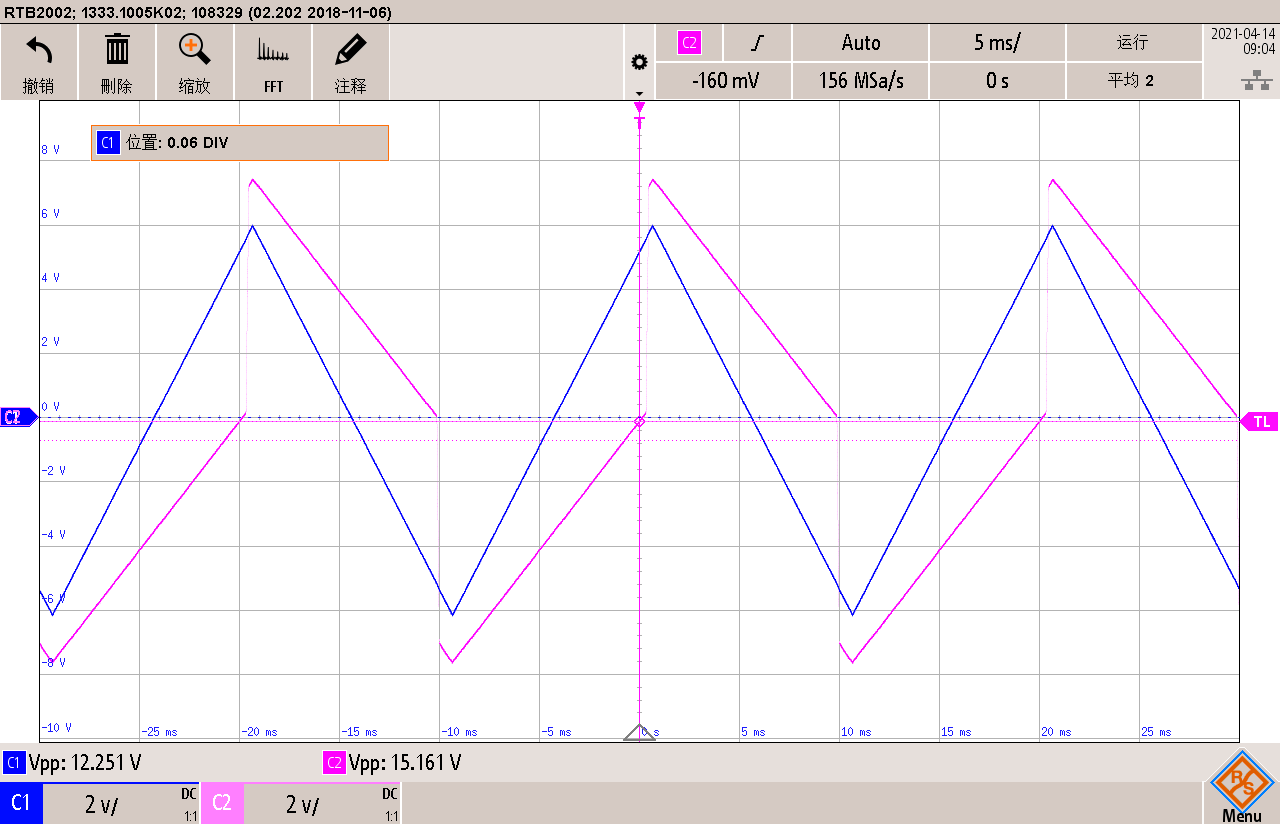
\includegraphics[width=3.5in]{H:/电子技术试验/4-15/4-15-18.png}
		\caption{同相滞回比较器的Ui和U+的波形} \label{fig:aa}
	\end{minipage}
  \end{figure}
    \begin{figure}[h]
		%\small
		\centering
		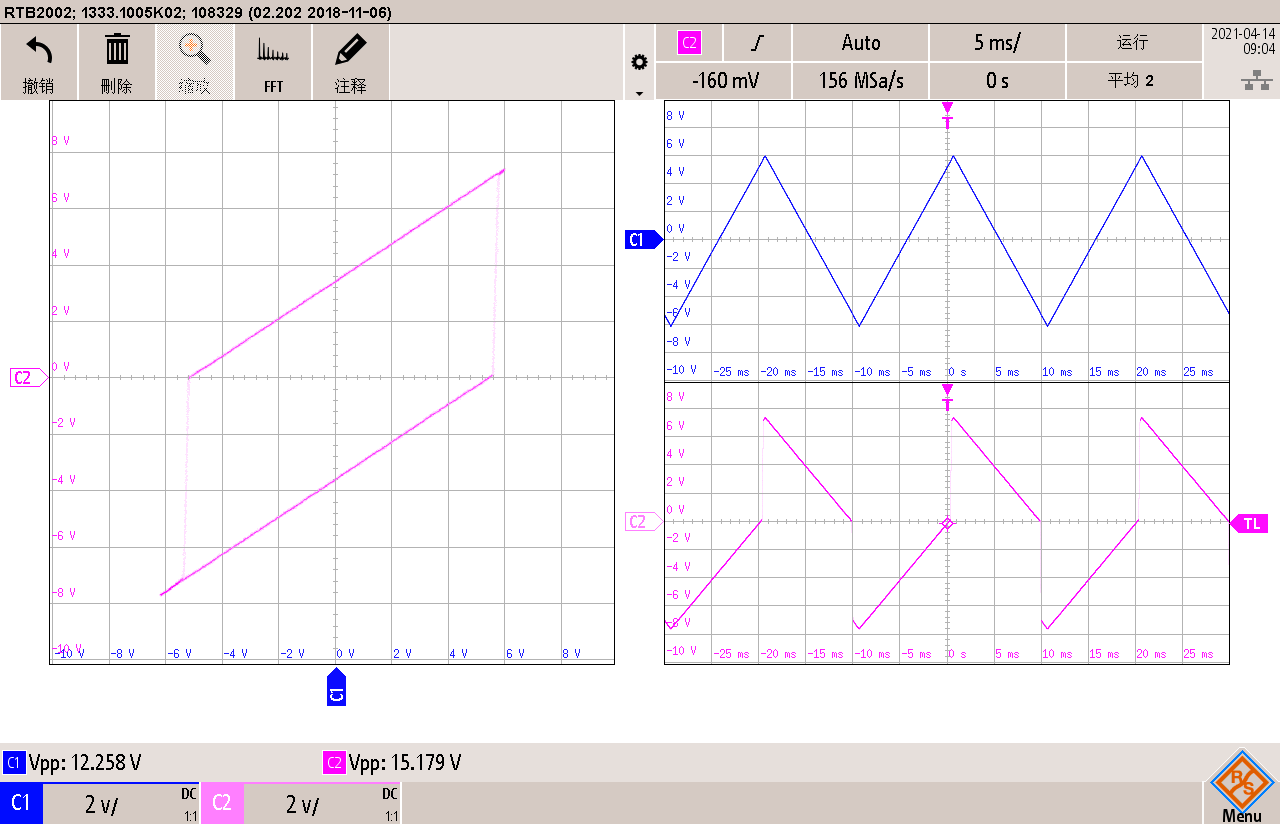
\includegraphics[width=3.5in]{H:/电子技术试验/4-15/4-15-19.png}
		\caption{同相滞回比较器的电压传输特性} \label{fig:aa}
	\end{figure}
	\par

	\section{\zihao{4} 实验设备和器材}
	(1)双踪示波器             \qquad \qquad \qquad \qquad \qquad  \qquad           1台\par
	(2)函数信号发生器          \qquad  \qquad \qquad \qquad       \qquad           1台\par
	(3)直流稳压电源             \qquad \quad \qquad \qquad \qquad \qquad           1台\par
	(4)模拟电路实验箱            \qquad  \qquad \qquad \qquad\qquad                1台\par
	(5)万用表                   \qquad  \qquad \qquad \qquad \qquad \qquad \qquad  1只\par
	(6)集成芯片LM358、电阻器\qquad\quad                                        若干

\section{结论}
(1)过零比较器可以用于检测一个输入值是否是零。原理是利用比较器对两个输入电压进行比较。当$U_i>$0时,输出$U_o=-(U_Z+U_D)$,当$U_i<0$时,$U_o=+(U_Z+U_D)$.其电压传输特性如图11所示.\par
(2)滞回比较器 $\Sigma$ 当$U_o$为正(记作$+U_{om}$),此时$\Sigma$点电压为\[U_H=\frac{R_2}{R_2+R_f}U_{om}\]  \par
当$U_i>U_H$后,即$U_o$由正变负(记作$-U_{om}$),此时$\Sigma$电压为\[U_H=-\frac{R_2}{R_2+R_f}U_{om}\]  \par

\section{思考题}
(1)图1所示电压比较器的$U_R$变化时其传输特性曲线如何变化?图3所示过零比较器输入电压Ui改接同相端,其传输特性曲线如何变化?\par
电压比较器的$U_R$变化时,电压传输特性使Uo为零的Ui发生变化,即Uo与Ui轴的交点变化.\par 
若过零比较器反接,则传输特性曲线是将原曲线中心对称变换的曲线。
\end{document}

